
\section{Finding Potential from the Electric Field}

\begin{comment}
This lab was originally written by Matt Trawick in spring 2015.  I found that students are really terrible at figuring out potential from electric field, and especially the idea of a reference potential.  The goal of this lab is to help them get better at this.  
\end{comment}

\makelabheader %(Space for student name, etc., defined in master.tex)

\vspace{0.4in}
\textbf{Introduction:}

In this lab, you will calculate and graph the electric potential $V$ from a known electric field $E$.  Keep in mind that the relationship between these two can be written as either a definite or indefinite integral:
\begin{displaymath}
\Delta V_{AB} = -\int_A^B{\vec{E} \cdot \vec{ds}} \qquad \textrm{ or } \qquad
V =-\int{\vec{E} \cdot \vec{ds}} 
\end{displaymath}
When evaluating the indefinite integral, remember that you always need a constant of integration, $+C$.  
\vspace{0.4in}

\begin{wrapfigure}[5]{r}{0.35\textwidth}
%\vspace{-0.2 in}
%    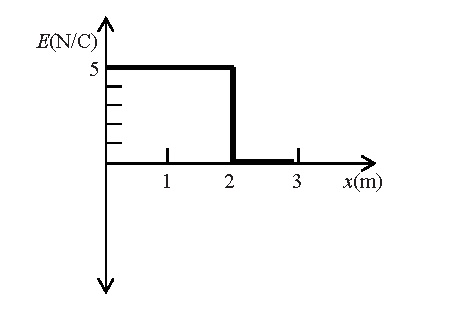
\includegraphics[width=0.4\textwidth]{finding_v_from_e/fig1.eps}
\hspace*{\fill}
\begin{lab_axis}[lab_grid,
	scale only axis = true,
	width={1.5in}, height={1.2in},
	xmin=0, xmax=3,
	ymin=-1, ymax=6,
	ylabel = {Field $E$ (N/C)},
	ytick = {-5,0,5,10},
	minor y tick num=4,
	minor x tick num=1,
	xlabel = {$x$ (m)},
	y0_line,
]
\addplot coordinates {(0,5) (2,5) (2,0) (3,0) };
\end{lab_axis}
\end{wrapfigure}

\textbf{Activity 1} 

The graph to the right shows a region of a uniform electric field $E(x)$.  

(a) If a positively charged particle starts at $x=0$ and is accelerated by the electric field to $x=2$, would the particle's kinetic energy $K$ \textit{increase} or \textit{decrease}?
\answerspace{0.7in}

(b) In part (a), would the particle's potential energy $U$ \textit{increase} or \textit{decrease}?
\answerspace{0.7in}

(c) Calculate the change in electric potential $\Delta V$ from $x=0$ to $x=2$. (Careful with your signs!)
\answerspace{0.9in}

(d) If the potential at the origin is defined as $V(0)=0$ volts (our ``reference''), what is the value of the potential $V$ at $x=2$?
\answerspace{0.7in}

\pagebreak
(e) Draw a graph of the electric potential on the axes below.  Include a scale on the vertical axis.
%\begin{center}
%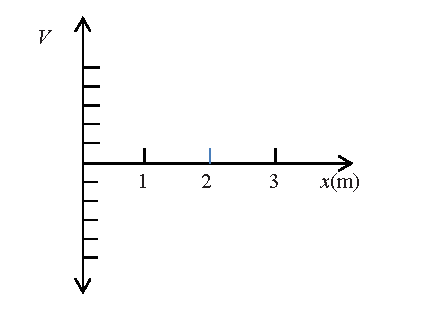
\includegraphics[width=0.4\textwidth]{finding_v_from_e/fig2.eps}
%\end{center}

\begin{lab_axis}*[lab_grid,
	scale only axis = true,
	width={3.0in}, height={1.5in},
	xmin=0, xmax=3,
	ymin=-4, ymax=4,
	ylabel = {Electric potential $V$},
	xlabel = {$x$ (m)},
	yticklabels = { , , },
	y0_line,
]
\end{lab_axis}

(f) Calculate the change in electric potential $\Delta V$ between $x=2$ and $x=3$.
\answerspace{0.5in}

(g) Recalling your answers to parts (d) and (f), what is the value of the electric potential $V$ at $x=3$?  (After you've answered this, you may want to go back and fix up your graph in part (e) to clarify $V(x)$ for $x>2$.
\answerspace{0.5in}

(h) Draw a graph showing the potential if we chose our reference so that $V(\infty)=0$ instead.  
%\begin{center}
%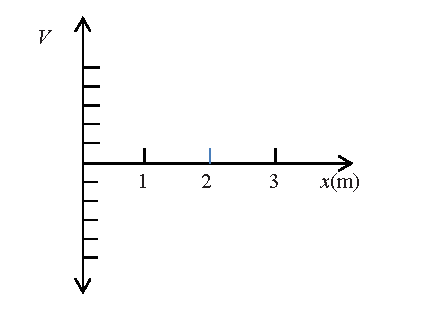
\includegraphics[width=0.4\textwidth]{finding_v_from_e/fig2.eps}
%\end{center}

\begin{lab_axis}*[lab_grid,
	scale only axis = true,
	width={3.0in}, height={1.5in},
	xmin=0, xmax=3,
	ymin=-4, ymax=4,
	ylabel = {Electric potential $V$},
	xlabel = {$x$ (m)},
	yticklabels = { , , },
	y0_line,
]
\end{lab_axis}

(i) Write an equation describing $V(x)$ based on your graph above.
\begin{displaymath}
V(x) = \begin{cases}
        \rule{1.3in}{0in}  & \textrm{when } 0<x<2\\
        \\
        \hspace{1.3in} & \textrm{when }  2 < x
        \end{cases}
\end{displaymath}
\answerspace{0.1in}

\pagebreak
\begin{wrapfigure}[5]{r}{0.5\textwidth}
%\vspace{-0.2 in}
%    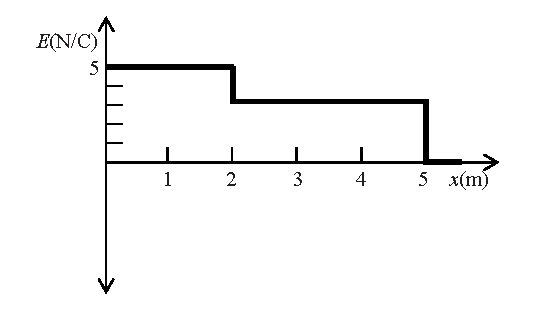
\includegraphics[width=0.5\textwidth]{finding_v_from_e/fig3.eps}
\hspace*{\fill}
\begin{lab_axis}[lab_grid,
	scale only axis = true,
	width={2.5in}, height={1.2in},
	xmin=0, xmax=6,
	ymin=-1, ymax=6,
	ylabel = {Field $E$ (N/C)},
	ytick = {-5,0,5,10},
%	ytick distance = 5,
	minor y tick num=4,
	xlabel = {$x$ (m)},
	y0_line,
]
\addplot coordinates {(0,5) (2,5) (2,3) (5,3) (5,0) (6,0)};
\end{lab_axis}
\end{wrapfigure}

\textbf{Activity 2} 

The graph to the right shows the electric field $E(x)$ in some other region.
(a) Calculate the change in electric potential $\Delta V$ between $x=0$ and $x=2$.
\answerspace{0.8in}

(b) Calculate the change in electric potential $\Delta V$ between $x=2$ and $x=5$.
\answerspace{0.7in}

(c) Draw a graph showing the potential, where the reference is $V(\infty)=0$.
%\begin{center}
%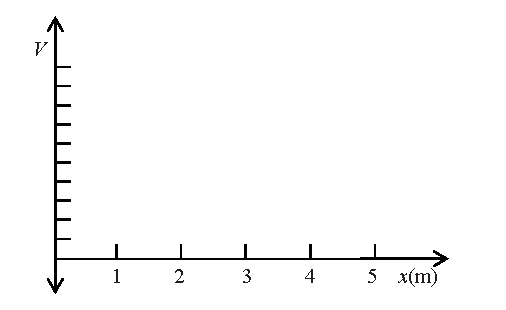
\includegraphics[width=0.45\textwidth]{finding_v_from_e/fig4.eps}
%\end{center}

\begin{lab_axis}*[lab_grid,
	scale only axis = true,
	width={3.0in}, height={1.8in},
	xmin=0, xmax=6,
	ymin=0, ymax=10,
	ylabel = {Electric potential $V$},
	xlabel = {$x$ (m)},
	ytick distance = 2,
	yticklabels = { , , },
	y0_line,
	minor tick num=1,
]
\end{lab_axis}


(d) Use the indefinite integral $V =-\int{\vec{E} \cdot \vec{ds}}$  to write an equation for $V(x)$ in the region $2<x<5$.  (Remember to include an integration constant, $+C$.  What equation should you use to find the value of $C$?)
\answerspace{1.0in}


(e) Write an equation describing $V(x)$ for all $x>0$.  It will be of the form
\begin{displaymath}
V(x) = \begin{cases}
        blah \, blah \, blah  & \textrm{when } 0<x<2\\
        yada \, yada \, yada & \textrm{when }  2<x<5\\
        something \, else & \textrm{when }  5 < x
        \end{cases}
\end{displaymath}

\answerspace{1.1in}

\pagebreak[2]
\textbf{Activity 3} 

The graph below shows the electric field $E(x)$ in yet another region.
%\begin{center}
%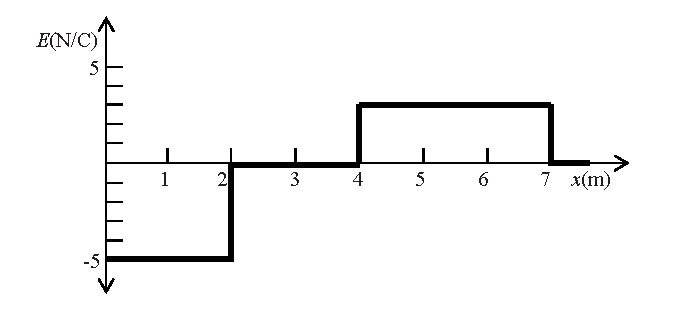
\includegraphics[width=0.6\textwidth]{finding_v_from_e/fig5.eps}
%\end{center}

\begin{lab_axis}*[lab_grid,
	scale only axis = true,
	width={3.5in}, height={1.7in},
	xmin=0, xmax=8,
	ymin=-6, ymax=6,
	ylabel = {Electric field $E$ (N/C)},
%	ytick = {-10,-5,0,5,10},
	ytick distance = 2,
	minor y tick num=1,
	xlabel = {$x$ (m)},
	y0_line,
]
\addplot coordinates {(0,-5) (2,-5) (2,0) (4,0) (4,3) (7,3) (7,0) (8,0)};
\end{lab_axis}

(a) Calculate the change in electric potential $\Delta V$ over each of the three regions shown.
\vspace{1.2in}

(b) Draw a graph of the potential $V(x)$, where the reference is $V(\infty)=0$.

\begin{lab_axis}*[lab_grid,
	scale only axis = true,
	width={3.5in}, height={1.5in},
	xmin=0, xmax=8,
	ymin=-4, ymax=4,
	ylabel = {Electric potential $V$},
	xlabel = {$x$ (m)},
	yticklabels = { , , },
	y0_line,
]
\end{lab_axis}

%\begin{center}
%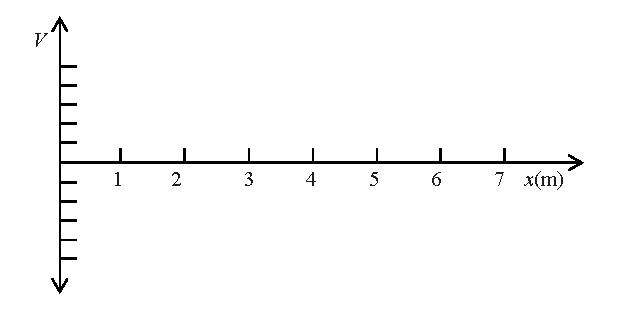
\includegraphics[width=0.6\textwidth]{finding_v_from_e/fig6.eps}
%\end{center}

(c) Is $V=0$ at $x=3$ (bearing in mind that the correct answer is ``No'')?
\answerspace{0.5in}

(d) In general, if $E=0$, does it follow that $V=0$?
\answerspace{0.5in}

(e) Where on your graph does $V=0$?  In general, if $V=0$, does it follow that $E=0$?
\answerspace{0.5in}

\pagebreak[2]
\begin{wrapfigure}[6]{r}{0.4\textwidth}
%\vspace{0.2 in}
%    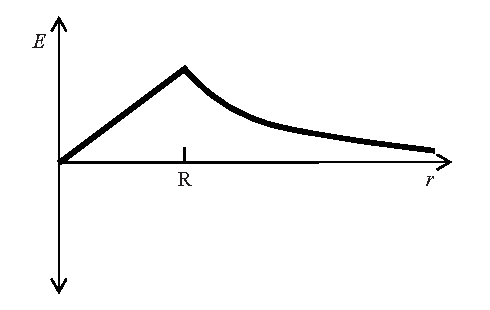
\includegraphics[width=0.4\textwidth]{finding_v_from_e/fig7.eps}
\hspace*{\fill}
\begin{lab_axis}[lab_noticks_2quads,
	scale only axis = true,
	algebraic_labels,
	width={2.2in}, height={1.3in},
	ymin=-0.3, ymax=1.5,
	xmin= 0, xmax = 4,
	ylabel = {$E$},
	xlabel = {$r$},
	xtick = {1},
	xticklabel = {$R$},
]
\addplot +[domain= 0 : 1] {x};
\addplot +[domain= 1 : 3.8] {1/x^2};
\end{lab_axis}
\end{wrapfigure}

\textbf{Activity 4} 

The graph to the right shows the electric field $E(r)$ near a uniformly charged sphere of radius $R$.  The electric field is given by
\begin{displaymath}
E(r) = \begin{dcases}
        \frac{k_eQr}{R^3}  &  0<r<R\\
        \frac{k_eQ}{r^2}  &  R<r
        \end{dcases}
\end{displaymath}

%(a) Use a definite integral to calculate $\Delta V$  between $r=R$ and $r=\infty$.
%\vspace{1.1in}

%(b) Use a definite integral to calculate $\Delta V$ between $r=0$ and $r=R$.
%\vspace{1.1in}

%Removed these last two parts, 2/14/2015. --MT.  These questions hurt more than they helped; students were trying to use the results of the definite integrals to figure out the constants of integration.  No big loss; it's not like this lab was too short before

%\vspace{0.5in}

(a) Draw a graph of the potential $V(r)$, using $V(\infty)=0$ as a reference.  (Hints: try telling yourself a story about how much potential energy you'd be adding to the system if you used your hand to push a small positive particle in from $r=\infty$.  Also remember that $E = - \frac{dV}{dr}$.  If you're not sure, sketch your best guess with a dotted line and go on to the next question.)
%\begin{center}
%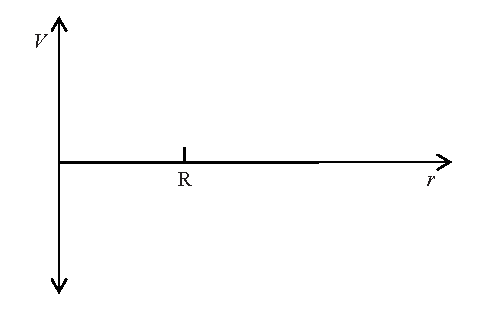
\includegraphics[width=0.5\textwidth]{finding_v_from_e/fig8.eps}
%\end{center}

\begin{lab_axis}*[lab_noticks_2quads,
	scale only axis = true,
	algebraic_labels,
	width={2.8in}, height={1.8in},
	xmin= 0, xmax = 4,
	ylabel = {$V$},
	xlabel = {$r$},
	xtick = {1},
	xticklabel = {$R$},
]
\end{lab_axis}

(b) Use indefinite integrals to write equations for $V(r)$ for each of the two regions, using $V(\infty)=0$ as your reference.  Be careful with signs, and remember the integration constants!
\answerspace{1.3in}

\vfill
(c) Now that you've calculated $V(r)$ exactly, go back and look at your graph in part (a).  Are your answers consistent?
